\documentclass{article}
\usepackage[margin=0.65in]{geometry}
\usepackage{enumitem}
\usepackage{graphicx}
\usepackage{hyperref}
\usepackage{titlesec}
\usepackage{xcolor}
\hypersetup{hidelinks}
\setlist[itemize]{leftmargin=1.5em,topsep=1pt,itemsep=0.5pt,parsep=0pt,partopsep=0pt}
\titlespacing*{\section}{0pt}{0.8ex}{0.4ex}
\setlength{\parindent}{0pt}
\setlength{\parskip}{0.3em}
\setlength{\textfloatsep}{5pt}
\setlength{\intextsep}{4pt}
\setlength{\abovecaptionskip}{2pt}
\setlength{\belowcaptionskip}{0pt}
\makeatletter
\renewcommand{\maketitle}{%
    \begin{center}
        {\Large\bfseries \@title\par}\vspace{0.1em}
        {\normalsize \@author\par}\vspace{0.1em}
        {\small \@date\par}
    \end{center}\vspace{0.4em}
}
\makeatother
% HJNotes-Tags: AI Infra, Top-K, BitonicSort
% HJNotes-Summary: Sequential top-K algorithms (sort, bubble, heap, quick select) with complexity, and parallel selection on GPU via bucket/radix sort.
\title{Top-K Algorithm}
\author{HJ}
\begin{document}
\maketitle
\section{Introduction}
% AGENT WARNING: only translate and polish the literal content, don't delete or add new stuff unless there are serious mistake.
Top-K is a classic algorithmic problem, nowadays widely used in AI. This essay only discusses the algorithm itself.

\section{Some Sequential Algorithms}
\begin{itemize}
    \item \textbf{Sort}: sort the $N$ elements and take the top $K$. Complexity: \textcolor{blue}{\textbf{$O(N \log N)$}}.
    \item \textbf{Bubble}: run $K$ bubble passes; each pass bubbles the next-largest element into place. Complexity: \textcolor{blue}{\textbf{$O(N K)$}}.
    \item \textbf{Heap}: scan the numbers while keeping the $K$ largest in a \textbf{min-heap} of size $K$. Complexity: \textcolor{blue}{\textbf{$O(N \log K)$}}.
    \item \textbf{Quick Select}: stop when a pivot lands at the $K$-th largest position; everything to its right is then the $K$ largest elements. Complexity: \textcolor{blue}{\textbf{$O(N)$}} on average, \textcolor{red}{\textbf{$O(N^2)$}} in the worst case.
\end{itemize}

\section{Some Parallel Algorithms}
Here are our two old friends, both have \textcolor{blue}{\textbf{$O(N)$}} work and \textcolor{blue}{\textbf{$O(\log N)$}} span.
\begin{itemize}
    \item \textbf{Bucket Sort}: parallels Quick Select --- apply a \textcolor{brown}{\textbf{parallel prefix sum}} over the bucket sizes (a sequential scan is also fine, since there are usually few buckets), find the ``pivot bucket'' that contains the $K$-th element, take every higher bucket outright, and recurse only on the pivot bucket.
    \item \textbf{Radix Sort (MSD)}: like radix buckets --- for example, take the highest 4 bits, which gives 16 buckets.
\end{itemize}

\section{Bitonic Sort, the GOAT}
\subsection{Algorithm analysis}
A sequence is \textbf{bitonic} if it first increases and then decreases, or is a cyclic rotation of such a sequence.

\textbf{Algorithm Description}:
\begin{itemize}
    \item Bitonic Sort: a descending and an ascending sequence of length $n$ can be merged and sorted by Bitonic Merge.
    \item Bitonic Merge: for a bitonic sequence of length $2n$, compare\&swap $x[i]$ with $x[i+n]$ so that $x[i] \le x[i+n]$; this yields 2 \textbf{bitonic} subsequences $x[0:n) \le x[n:2n)$, and the bitonic property is preserved by Batcher's theorem. After \textbf{recursively doing so}, we get a sorted sequence.
\end{itemize}

\textbf{Work \& Span}: Obviously, Bitonic Sort is \textcolor{blue}{\textbf{extremely highly parallelizable}}: every compare-and-swap can be done by a single thread. Although its total work is even worse than merge sort's, its span is \textcolor{blue}{\textbf{polylogarithmic}}.

There is \underline{no early termination for top-K}, but good enough.

\begin{figure}[!ht]
    \centering
    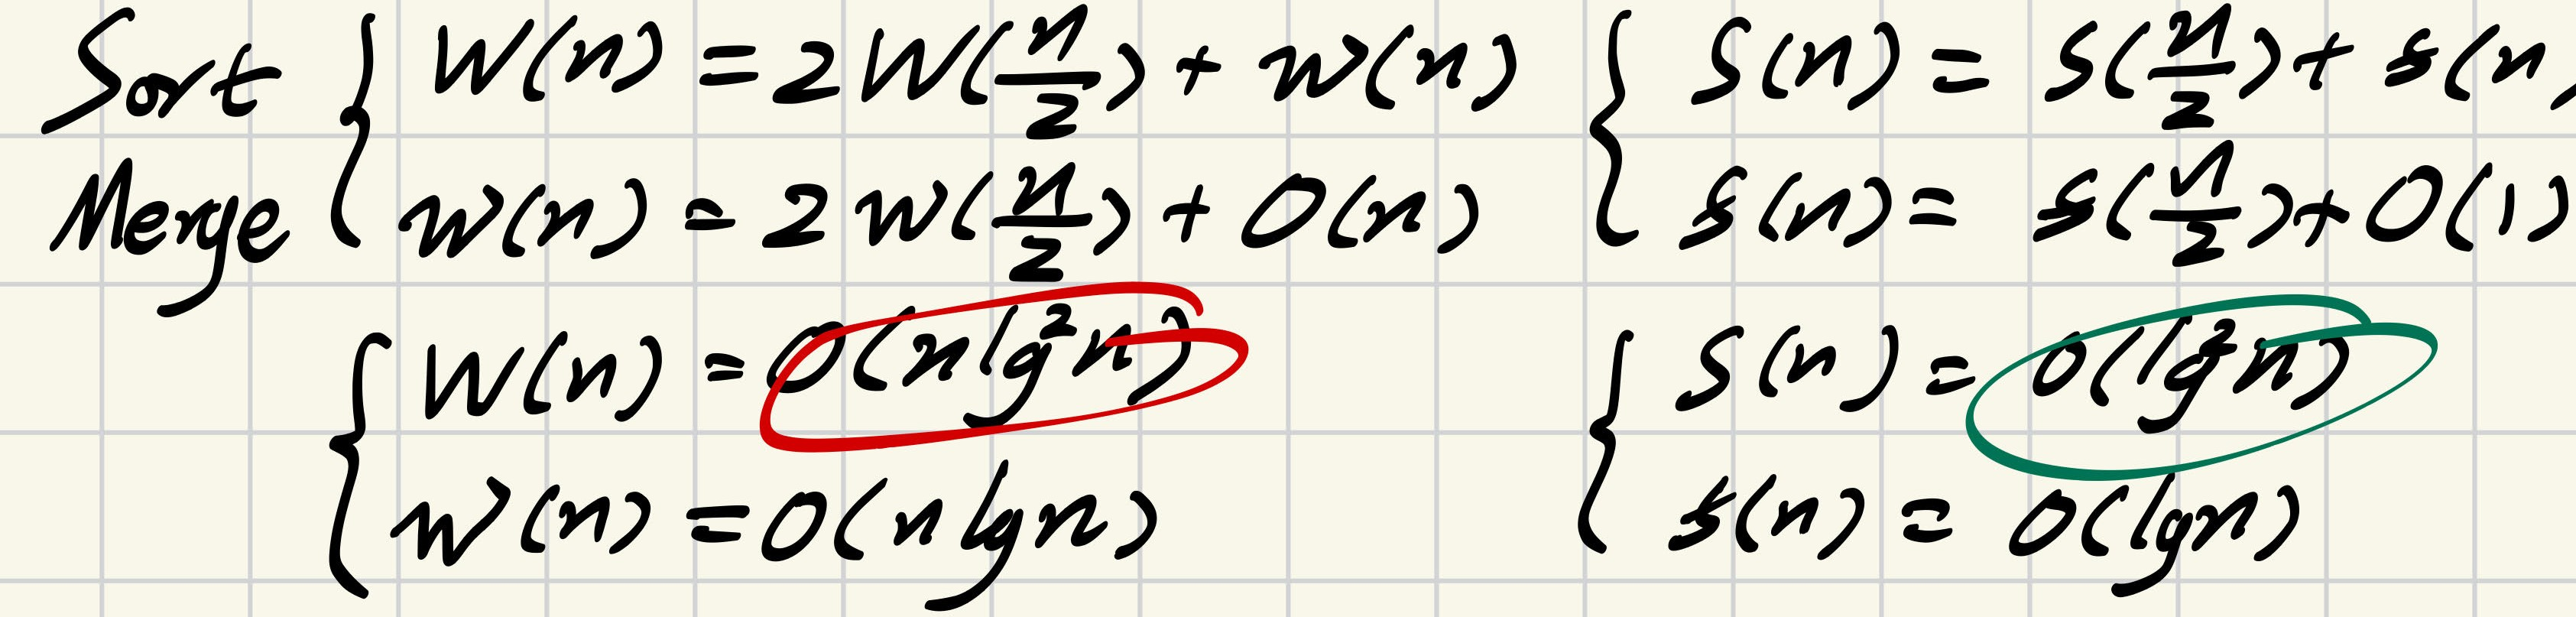
\includegraphics[width=0.58\linewidth,height=0.3\textheight,keepaspectratio]{bitonic-work-span-analysis.jpg}
    \caption{Bitonic Sort work and span analysis.}
\end{figure}

\begin{figure}[!ht]
    \centering
    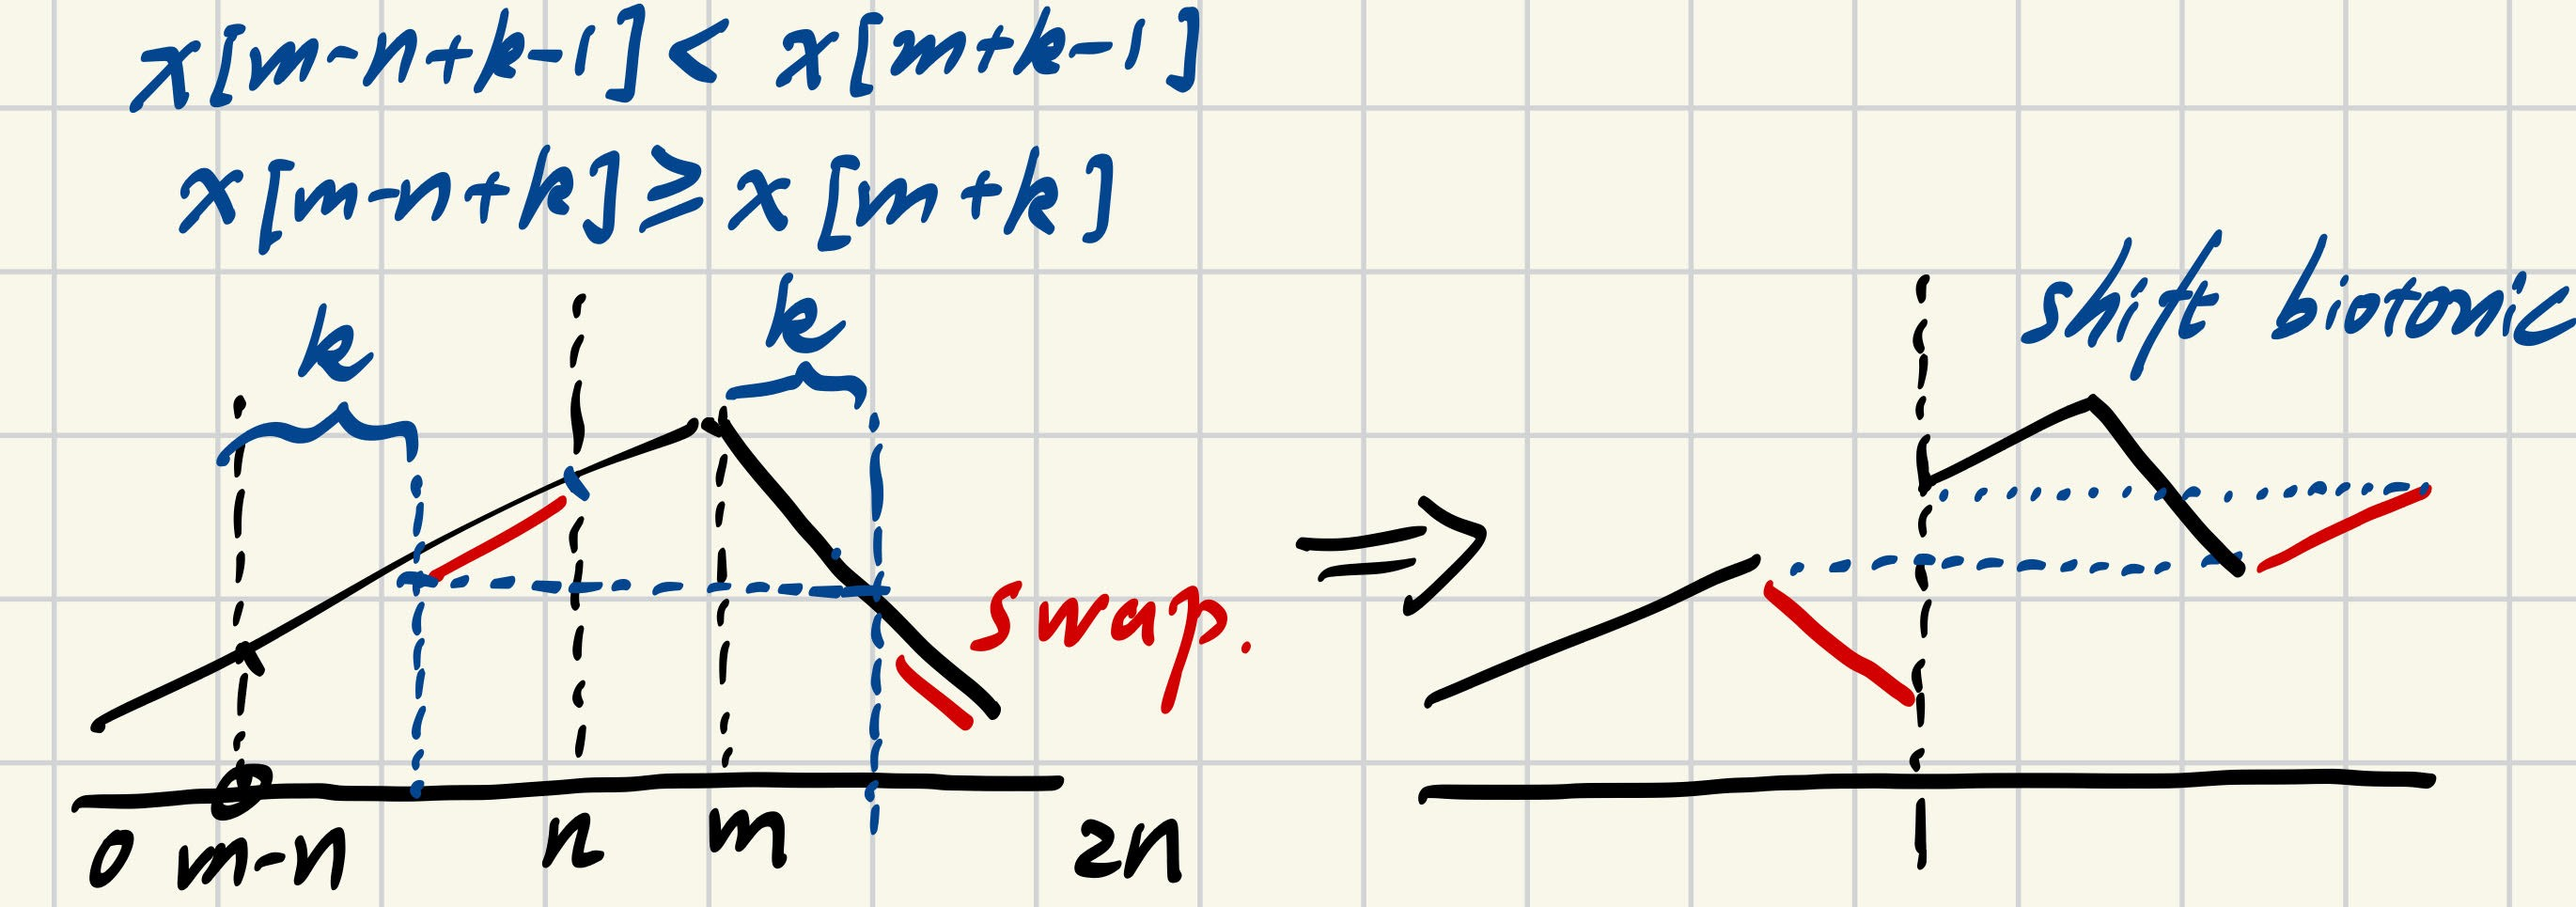
\includegraphics[width=0.58\linewidth,height=0.3\textheight,keepaspectratio]{Batcher-Therom-Demonstration.jpg}
    \caption{Batcher's theorem}
\end{figure}

\subsection{Calculation Example}
We write Sort in bottom-up order since it works after branches, and Merge in top-down order since it works before branches.

\begin{figure}[!ht]
    \centering
    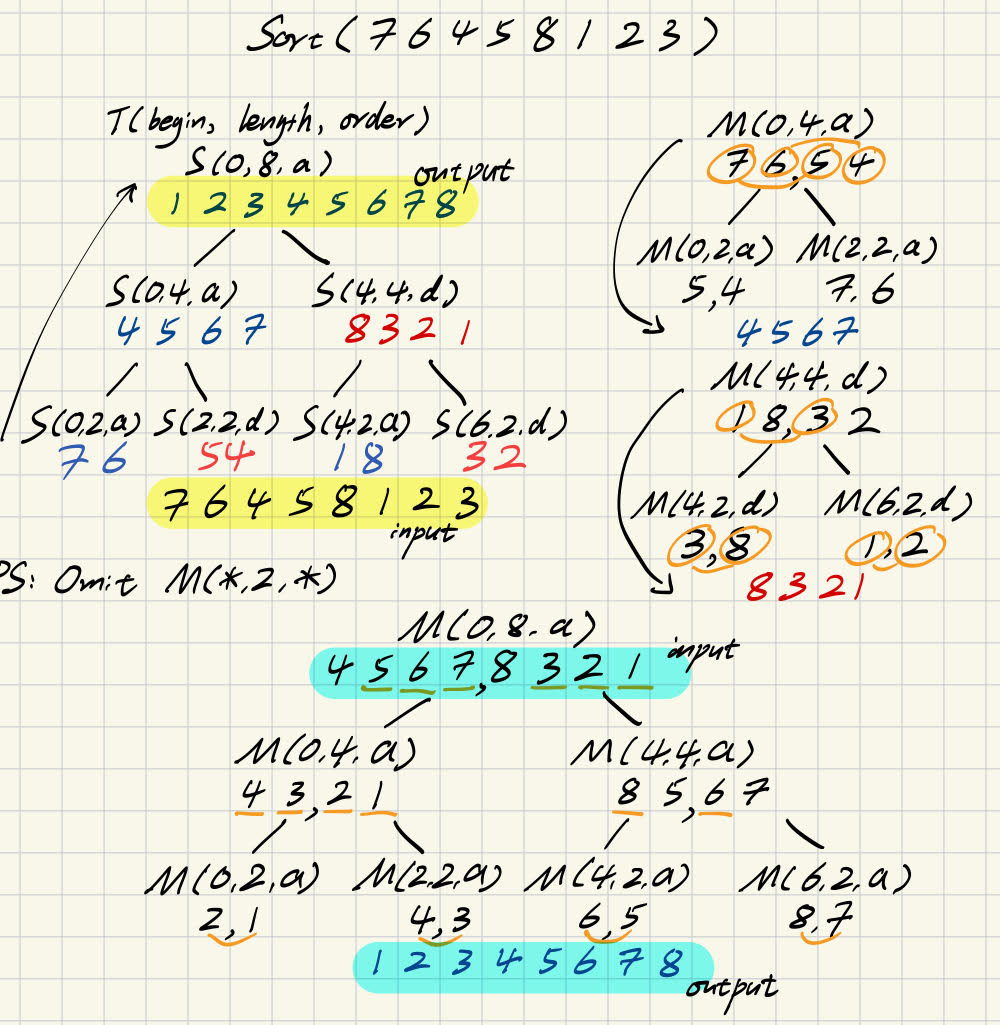
\includegraphics[width=0.73\linewidth,height=\textheight,keepaspectratio]{caculation-manuscript.jpg}
    \caption{The whole calculation procedure}
\end{figure}

\textcolor{red}{TODO: Add Cuda details?}

\textcolor{red}{XXX: the Batcher's Theorem Illustration only demonstrate a single cases, we need more for the shift cases, or shall we just skip the math burden?}

\end{document}
